%%%%%%%%%%%%%%%%%%%%%%%%%%%%%%%%%%%%%%%%%
% Beamer Presentation
% LaTeX Template
% Version 1.0 (10/11/12)
%
% This template has been downloaded from:
% http://www.LaTeXTemplates.com
%
% License:
% CC BY-NC-SA 3.0 (http://creativecommons.org/licenses/by-nc-sa/3.0/)
%
%%%%%%%%%%%%%%%%%%%%%%%%%%%%%%%%%%%%%%%%%

%----------------------------------------------------------------------------------------
%	PACKAGES AND THEMES
%----------------------------------------------------------------------------------------

\documentclass{beamer}

\mode<presentation> {

% The Beamer class comes with a number of default slide themes
% which change the colors and layouts of slides. Below this is a list
% of all the themes, uncomment each in turn to see what they look like.

%\usetheme{default}
%\usetheme{AnnArbor}
%\usetheme{Antibes}
%\usetheme{Bergen}
%\usetheme{Berkeley}
%\usetheme{Berlin}
%\usetheme{Boadilla}
%\usetheme{CambridgeUS}
%\usetheme{Copenhagen}
%\usetheme{Darmstadt}
%\usetheme{Dresden}
%\usetheme{Frankfurt}
%\usetheme{Goettingen}
%\usetheme{Hannover}
%\usetheme{Ilmenau}
%\usetheme{JuanLesPins}
%\usetheme{Luebeck}
\usetheme{Madrid}
%\usetheme{Malmoe}
%\usetheme{Marburg}
%\usetheme{Montpellier}
%\usetheme{PaloAlto}
%\usetheme{Pittsburgh}
%\usetheme{Rochester}
%\usetheme{Singapore}
%\usetheme{Szeged}
%\usetheme{Warsaw}

% As well as themes, the Beamer class has a number of color themes
% for any slide theme. Uncomment each of these in turn to see how it
% changes the colors of your current slide theme.

%\usecolortheme{albatross}
%\usecolortheme{beaver}
%\usecolortheme{beetle}
%\usecolortheme{crane}
%\usecolortheme{dolphin}
%\usecolortheme{dove}
%\usecolortheme{fly}
%\usecolortheme{lily}
%\usecolortheme{orchid}
%\usecolortheme{rose}
%\usecolortheme{seagull}
%\usecolortheme{seahorse}
%\usecolortheme{whale}
%\usecolortheme{wolverine}

%\setbeamertemplate{footline} % To remove the footer line in all slides uncomment this line
\setbeamertemplate{footline}[page number] % To replace the footer line in all slides with a simple slide count uncomment this line

\setbeamertemplate{navigation symbols}{} % To remove the navigation symbols from the bottom of all slides uncomment this line
}

\usepackage[utf8]{inputenc}
\usepackage[english,russian]{babel}
\usepackage{amsmath,mathrsfs,mathtext}
\usepackage{graphicx, epsfig}
\usepackage{caption}
\usepackage{subfig}
\usepackage{amsmath}

\DeclareMathOperator*{\argmin}{arg\,min}
\DeclareMathOperator*{\argmax}{arg\,max}

\usepackage{graphicx} % Allows including images
\usepackage{booktabs} % Allows the use of \toprule, \midrule and \bottomrule in tables
%\usepackage {tikz}
\usepackage{tkz-graph}
\GraphInit[vstyle = Shade]
\tikzset{
  LabelStyle/.style = { rectangle, rounded corners, draw,
                        minimum width = 2em, fill = yellow!50,
                        text = red, font = \bfseries },
  VertexStyle/.append style = { inner sep=5pt,
                                font = \normalsize\bfseries},
  EdgeStyle/.append style = {->, bend left} }
\usetikzlibrary {positioning}
%\usepackage {xcolor}
\definecolor{beamer@blendedblue}{RGB}{31,96,49}
%----------------------------------------------------------------------------------------
%	TITLE PAGE
%----------------------------------------------------------------------------------------

\title[Short title]{Задача поиска символов в текстах} % The short title appears at the bottom of every slide, the full title is only on the title page

\author{Северилов Павел Андреевич} % Your name
\institute[Московский физико-технический институт] % Your institution as it will appear on the bottom of every slide, may be shorthand to save space
{
Московский физико-технический институт \\ % Your institution for the title page
\medskip
}
\date{Курс: Численные методы обучения по прецедентам \\(практика, В.\,В. Стрижов)/Группа 674, весна 2019} % Date, can be changed to a custom date

\begin{document}

%------------------------------------------------

	\begin{frame}
		\titlepage
	\end{frame}
	
	%-----------------------------------------------------------------------------------------------------
	\begin{frame}{Цель исследования}
	\begin{block}{Проблема}
		Современные модели для обработки текстов воспринимают высказывания буквально, и различные средства художественной выразительности, в частности, символы, метафоры, аллегории и др. не интерпретируются ими верным образом.
	\end{block}
	
	\begin{block}{Цель работы}
		Получить оптимальную модель для определения неоднозначности в высказываниях.
	\end{block}
	
	\end{frame}
	%----------------------------------------------------------------------------------------------------------
	\begin{frame}{Постановка задачи}
			\begin{block}{Sequence labeling} Дано предложение \textbf{X}, разделенное на слова: $\{x_1, x_2, \cdots, x_n\}$. Требуется построить последовательность двоичных меток (labels) $\{l_1, l_2, \cdots, l_n\}$, которые идентифицируют наличие неоднозначности/символа в каждом слове  $x_i$
			\end{block}
		
			\begin{block}{Классификация} Аналогично дано предложение \textbf{X}, разделенное на части: $\{x_1, x_2, \cdots, x_n\}$. Требуется для целевой переменной $i$ предсказать отношение $x_i$ к классу символ или не символ, соответственно 1 и 0. 
			\end{block}
	\end{frame}
	%----------------------------------------------------------------------------------------------------------
			\begin{frame}{Базовый алгоритм}
				\begin{figure}[H]
					\centering
					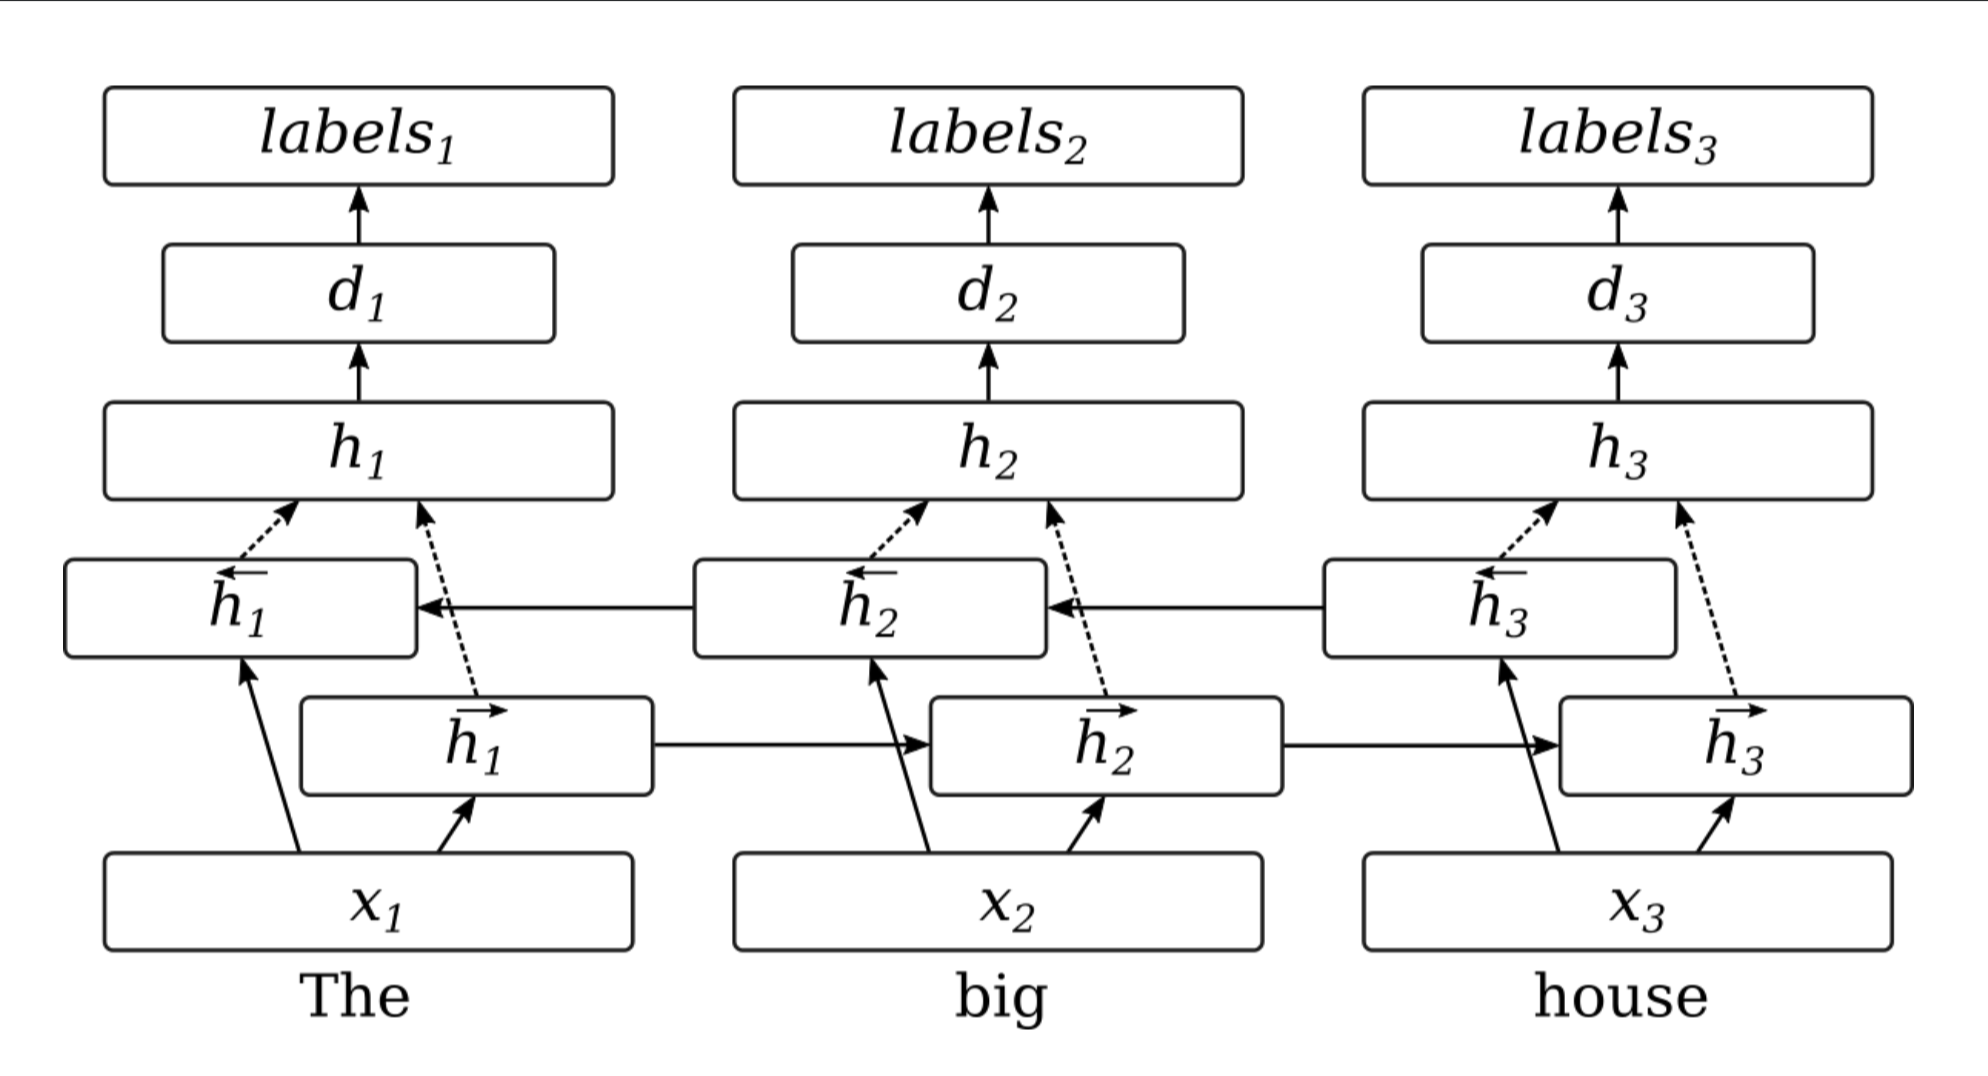
\includegraphics[width=0.60\textwidth]{./pics/BiLSTM}
					\caption{Схема базовой модели BiLSTM}
				\end{figure}
				\begin{block}{ Представления в LSTM-сети} 
					$$\overrightarrow{h_t} = \text{LSTM}(x_\text{t}, \overrightarrow{h_{t-1}})~~~~~
					\overleftarrow{h_t} = \text{LSTM}(x_\text{t}, \overleftarrow{h_{t+1}})~~~~
					h_\text{t} = [\overrightarrow{h_\text{t}};\overleftarrow{h_\text{t}}]$$
					Скрытый слой нелинейности:
					$d_\text{t} = tanh(W_\text{d}h_\text{t}),$
					где $\textbf{W}_\text{d}$ -- весовая матрица между слоями.
				\end{block}
			\end{frame}
	%----------------------------------------------------------------------------------------------------------
	
	\begin{frame}{ Итоговая задача оптимизации}
	Нормированное распределение вероятностей по всем возможным меткам для каждого слова (softmax):
			
			$$\mathbb{P}(y_t = k| d_t) = \cfrac{e^{W_kd_\text{t}}}{\sum_{\tilde{k}\in K}e^{W_\tilde{k}d_\text{t}}},$$
			где $\mathbb{P}(y_t = k| d_t)$ -- вероятность того, что метка t-ого слова $y_t$ будет k ($K$ -- множество всевозможных меток), $\textbf{W}_k$ -- k-ая строка весовой матрицы $\textbf{W}$. 

			Для оптимизации модели используется минимизация функции
			$$\mathcal{L} = -\sum_{t=1}^{T}\log(\mathbb{P}(y_t|d_t))$$
			
			Т.е. решается данная задача: 
			$$\boxed{\textbf{W}^* = \underset{W}{\text{argmin}}(\mathcal{L}(\textbf{W}))}$$
	\end{frame}
		%----------------------------------------------------------------------------------------------------------
		\begin{frame}{Вычислительный эксперимент}
				\begin{block}{Модели}
					Предлагается сравнить следующие модификации базового алгоритма:
					\begin{enumerate}
						\item Базовая BiLSTM нейронная сеть
						\item BiLSTM нейронная сеть с CRF (Conditional random field)
						\item BiLSTM нейронная сеть с Attention
					\end{enumerate}
				\end{block}
				
		\begin{block}{Данные}
			\begin{enumerate}
				\item MOH датасет с метафорами (eng)
				\item VU Amsterdam Metaphor Corpus (eng)
				\item Собственная разметка русских текстов (НОВИНКА)
			\end{enumerate}
		\end{block}
	
		\end{frame}

	%----------------------------------------------------------------------------------------------------------
	\begin{frame}{Результаты эксперимента: Loss график}
		\begin{figure}[H]
			\centering
			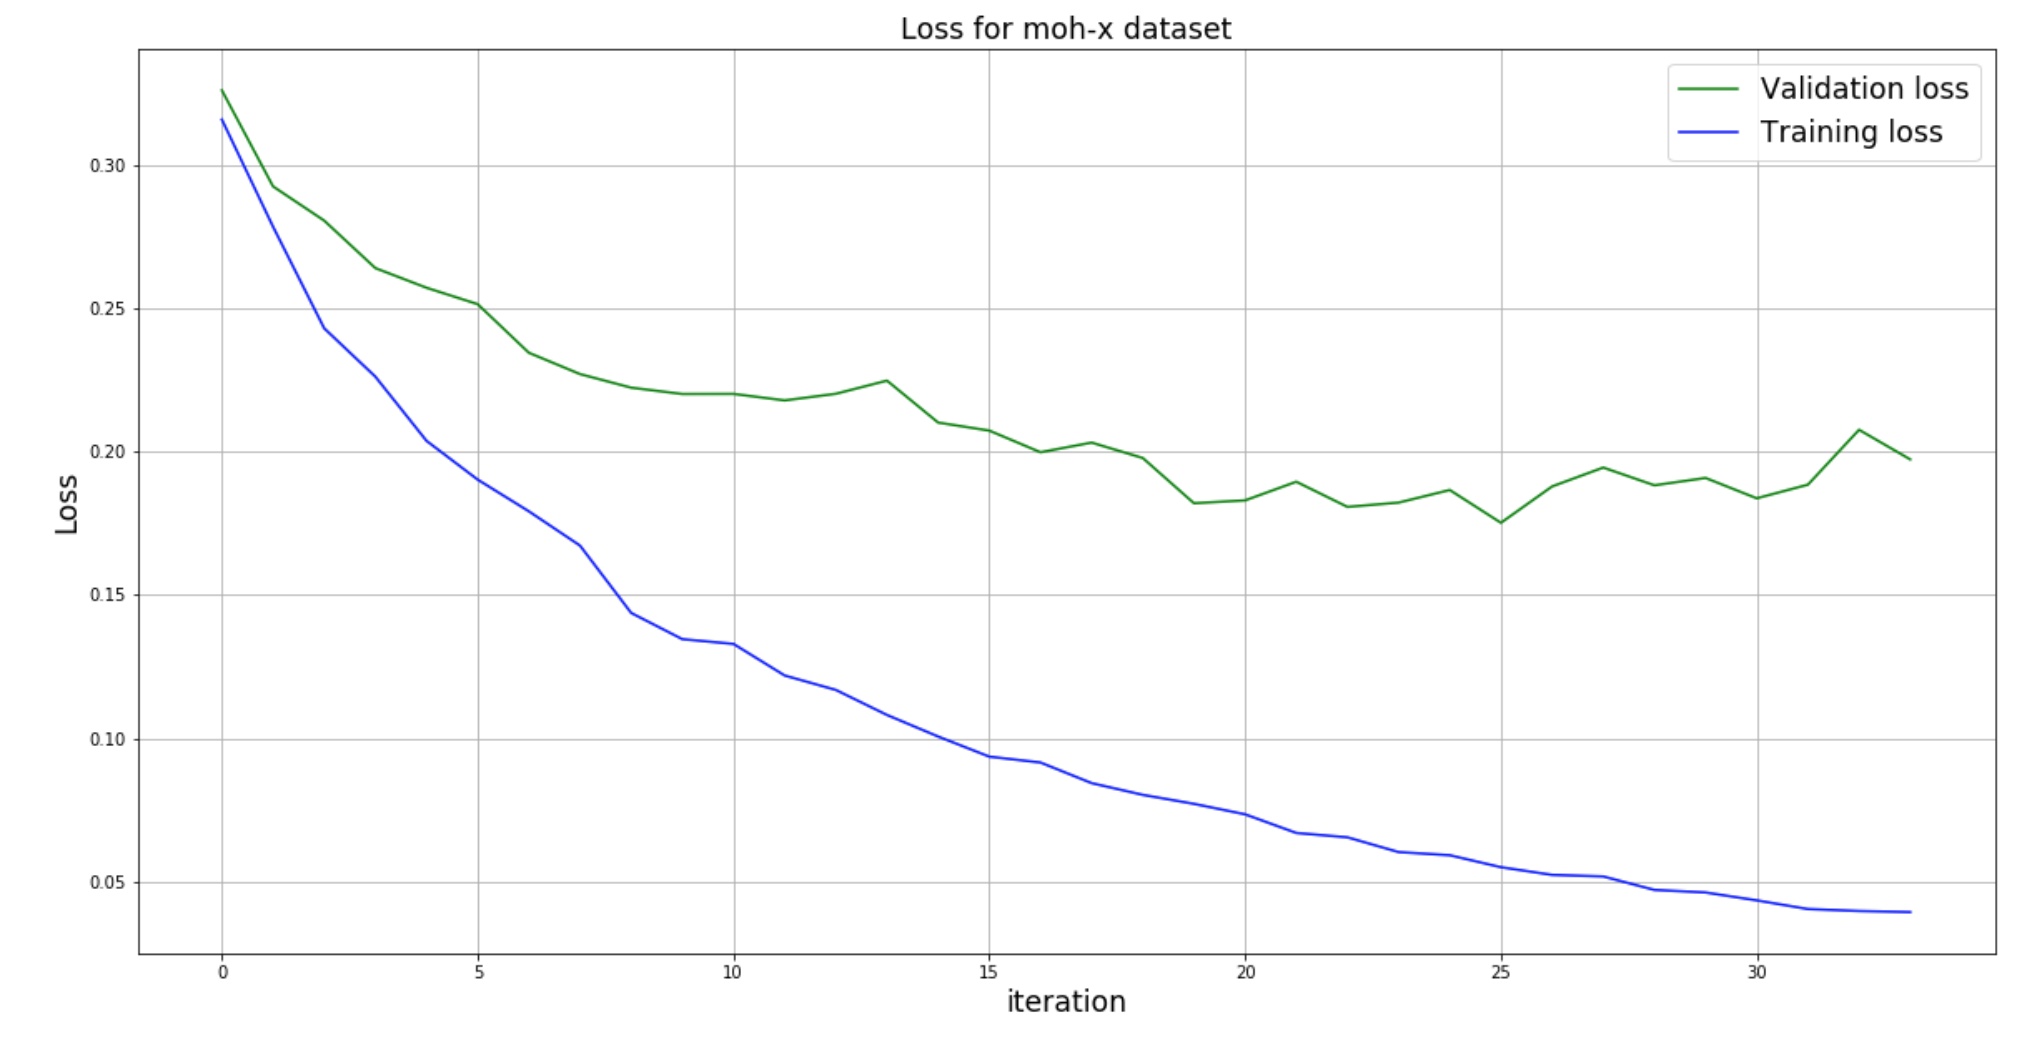
\includegraphics[width=1.0\textwidth]{./pics/loss}
		\end{figure}
	\end{frame}
	%----------------------------------------------------------------------------------------------------------
		\begin{frame}{Результаты эксперимента: F1 мера}
			\begin{figure}[H]
				\centering
				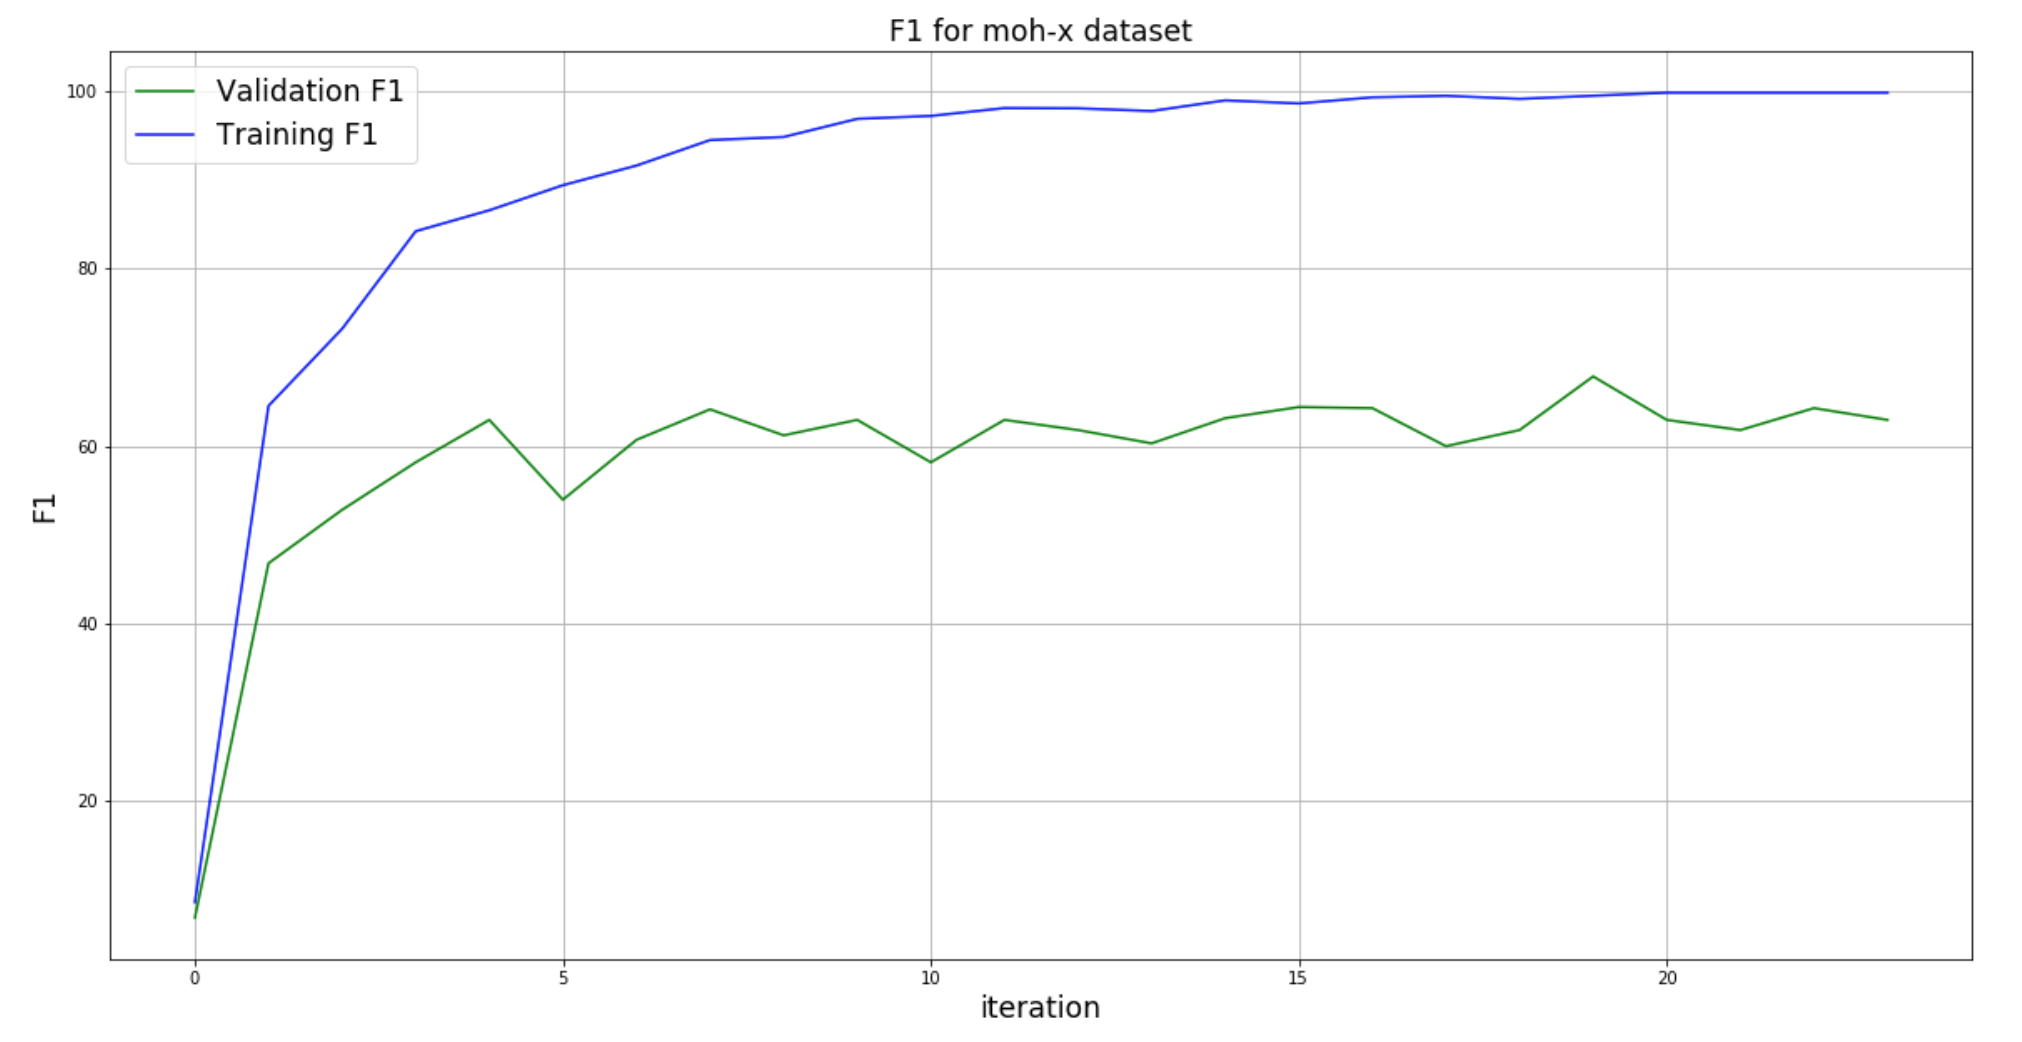
\includegraphics[width=1.0\textwidth]{./pics/F1}
			\end{figure}
		\end{frame}
		
		%----------------------------------------------------------------------------------------------------------
		\begin{frame}{Результаты эксперимента: Качество}
			\begin{center}
					\textbf{	Качество алгоритма после 30 эпох обучения:}
		\begin{itemize}
			\item Precision on MOH =  \textbf{64}.14203612479474
			\item Recall on MOH =  \textbf{67}.85714285714286
			\item F1 on MOH =  \textbf{65}.8939014202172
			\item Accuracy on MOH =  \textbf{69}.27083333333333
		\end{itemize}
			\end{center}
		\end{frame}
		%----------------------------------------------------------------------------------------------------------
	\begin{frame}{Заключение}
		\begin{itemize}
			\item Алгоритм sequence labeling хорошо подходит для поиска символов в тексте
			\item Сравнены результаты работ нескольких моделей: наилучшая – ?
			\item Главная проблема эксперимента -- мало данных
			\item Качество заметно улучшится при увеличении выборки
			\item Предложенные модели могут быть применены для определения не только каких-то конкретных неоднозначностей в тексте, а в целом для всех видов символов
			\item Для русскоязычных текстов данная задача никак до этого не решалась
		\end{itemize}
	\end{frame}
	%----------------------------------------------------------------------------------------------------------

\end{document}
